\documentclass[tikz,margin=5pt,12pt]{standalone}
\usepackage{tikz}
\usepackage{xparse}
\usetikzlibrary{calc,arrows.meta}

% Default styles definition
% This has to be here, because is executed when the library is load, before command invocation.
% This is very important for avoid the re-definition of user styles
\tikzset{% 
    prim-Dim/.style={%
      >={Latex[length=3mm, width=1.5mm]}, % Arrow head proprieties
      very thin,                          % Line style
      font=\footnotesize,                 % Dimension line text size
    },
    prim-DimNode/.style={prim-Dim,
      fill=white,                         % Fill with color background, by default white
      inner sep=0pt,                      % Space to the line 
      outer sep=0pt,                      % Space to the line 
    },
    Dimension/.style={},                  % Empty style for user use
    DimNode/.style={},                    % Empty style for user use
}

\makeatletter
\NewDocumentCommand{\Cote}{%
%-------------------------------------------------------------------------------------------%
%                                 Input Parameters                                          %
%-------------------------------------------------------------------------------------------%
% Type? | brackets | Default |                  Mean
    s                        % #1 Is the star. With star the arrow is external.
    D       <>         {o}   % #2 Label position (it's a point)
    O                 {10mm}  % #3 Offset of dimension line
    m                        % #4 First point
    m                        % #5 Second point
    D       <>         {o}   % #6 Third point. It's useful in angle dimension
    m                        % #7 Label
    D       <>         {o}   % #8 h: Horizontal, v: Vertical, r: Radius, a: Angle, o: Oblique
    O                  {}    % #9 Parameters for include in tikzset
%-------------------------------------------------------------------------------------------%
}{%

{%%%%%%%%%%%%%%%%%%%%%%%%%%%%%%%%%  Start the body of Command  %%%%%%%%%%%%%%%%%%%%%%%%%%%%%%
  
  % User defined styles
  \tikzset{#9}

  % Total styles
  \tikzset{%
    Dim/.style  ={prim-Dim,Dimension},
    Node/.style ={prim-DimNode,DimNode},
  }

  %---------------------------------- Coordinates calculation -------------------------------
  % (@0) -> Is the label position
  % (@1) -> Is the first limit line point
  % (@2) -> Is the second limit line point
  % (@3) -> Is the first dimension line point 
  % (@4) -> Is the second dimension line point 

  \coordinate (@1) at #4;
  \coordinate (@2) at #5;

  \if #8v % Vertical dimension
    \coordinate (@0) at ($($#4!.5!#5$) + (#3,0)$); 
    \coordinate (@3) at (@0|-@1);
    \coordinate (@4) at (@0|-@2);

  \else\if #8h % Horizontal dimension
    \coordinate (@0) at ($($#4!.5!#5$) + (0,#3)$); 
    \coordinate (@3) at (@0-|@1);
    \coordinate (@4) at (@0-|@2);

  \else\if #8r % Radial dimension
      \coordinate (@3) at (@1);
      \coordinate (@4) at (@2);

  \else\if #8a % Angular dimension
      \coordinate (@4) at ($#6!#3!#5$);
      \coordinate (@3) at ($#6!#3!#4$);

  \else\if #8o % Oblique dimension   
      \coordinate (@4) at ($#5!#3!90:#4$);
      \coordinate (@3) at ($#4!#3!-90:#5$);

  \fi\fi\fi\fi\fi

  %-------------------------------------- Put limit lines -----------------------------------

  \if #8r % If is radius dimension
    \draw[Dim, fill] (@1) circle (0.3mm);
    \draw[Dim] ($(@1) + (0,1.5mm)$) -- ($(@1) + (0,-1.5mm)$);
    \draw[Dim] ($(@1) + (1.5mm,0)$) -- ($(@1) + (-1.5mm,0)$);

  \else % If isn't radius dimension
    \draw[Dim, shorten >= 1mm, shorten <= -3mm] (@3) -- (@1);
    \draw[Dim, shorten >= 1mm, shorten <= -3mm] (@4) -- (@2);

  \fi

  %----------------------------------- Put dimension lines -----------------------------------

  \IfBooleanTF #1 {% Con asterisco

    % \if #8a

    \draw[Dim,-] (@3) -- (@4) node[Node] at ($ 0.5*(@3) + 0.5*(@4) $) {#7\strut};
    \draw[Dim,<-] (@3) -- ($(@3)!-5mm!(@4)$);   
    \draw[Dim,<-] (@4) -- ($(@4)!-5mm!(@3)$);   

  }{%Sin asterisco

  \if #8a % Angular dimension
    \draw[Dim, <-> ] (@4) to[bend right] node[Node] {#7\strut} (@3);
  \else\if #8r
    \draw[Dim, ->] (@3) -- (@4) node[Node] at ($ 0.5*(@3) + 0.5*(@4) $) {#7\strut};
  \else
    \draw[Dim, <->] (@3) -- (@4) node[Node] at ($ 0.5*(@3) + 0.5*(@4) $) {#7\strut};
  \fi\fi

  }}
}
\makeatother


\usetikzlibrary{patterns}
\begin{document}
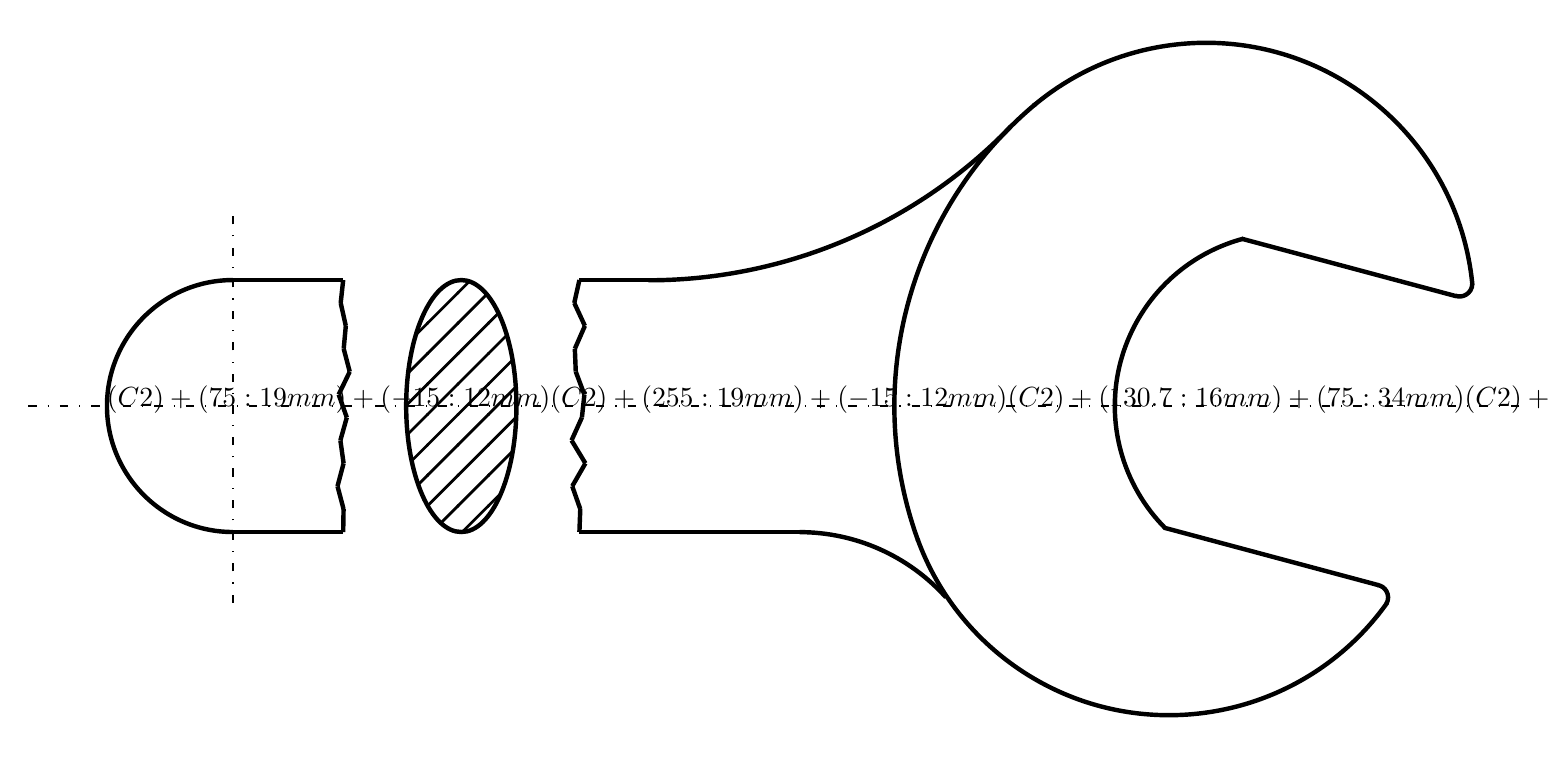
\begin{tikzpicture}

%-------------------- Irregular line  ------------------------------
\NewDocumentCommand{\irregularline}{%
  O     {2mm}   % Amplitude of irregularity. Optional. Default value = 2mm
  m             % First point
  m             % Second point
  D   <> {20}   % Number of peaks. Optional. Default value = 20
  O       {}    % Draw options
}{{%
    \coordinate (old) at #2;
    \foreach \i in {1,2,...,#4}{
      % This crazy line means:
      % draw from old to [ (i% from #2 to #3) + (#1*rand perpendicular to #2-#3) - (#2 because was added twice) ]
      \draw[#5] (old) -- ($ ($#2!\i/(#4+1)!#3$) + ($#2!#1*rand!-90:#3$) - ($#2$) $) coordinate (old);
    }
    \draw[#5] (old) -- #3;
  }}

%-------------------- Pattern definition  ------------------------------
\tikzset{%
  hatch distance/.store in=\hatchdistance, 
  hatch distance=10pt,
  hatch thickness/.store in=\hatchthickness,
  hatch thickness=1pt,
}
\pgfdeclarepatternformonly[\hatchdistance,\hatchthickness]{section}
{\pgfqpoint{0pt}{0pt}}
{\pgfqpoint{\hatchdistance}{\hatchdistance}}
{\pgfpoint{\hatchdistance-1pt}{\hatchdistance-1pt}}%
{%
  \pgfsetlinewidth{\hatchthickness}
  \pgfpathmoveto{\pgfqpoint{0pt}{0pt}}
  \pgfpathlineto{\pgfqpoint{\hatchdistance}{\hatchdistance}}
  \pgfusepath{stroke}
}

%--------------------  Base figure  ------------------------------
\tikzset{%
  fix/.style = {ultra thick},
  tmp/.style = {very thin, green},
  ctr/.style = {loosely dashdotted},
  dot/.style = {very thin, red},
}

\def\Ra{16mm}
\def\Rb{50mm}

\coordinate (C1) at (16mm,0mm);
\coordinate (C2) at (150mm,0mm);

% Body
\draw[fix] (\Ra,\Ra) -- (30mm,\Ra);
\draw[fix] (\Ra,-\Ra) -- (30mm,-\Ra);
\draw[fix] (60mm,\Ra) -- (69mm,\Ra);
\draw[fix] (60mm,-\Ra) -- (88mm,-\Ra);
\irregularline[1mm]{(30mm,\Ra)}{(30mm,-\Ra)}<10>[fix]
\irregularline[1mm]{(60mm,\Ra)}{(60mm,-\Ra)}<10>[fix]

%Body curves
\draw[fix] ($(C2) + (135.45:\Rb+64mm) + (316:64mm)$) arc (316:270:64mm); 
\draw[fix] ($(C2) + (199.2:16mm) + (217.3:59mm) + (42:25mm)$) arc (42:90:25mm); 
% \draw[dot] ($(C2) + (135.4:\Rb+64mm)$) circle (0.1mm); 
% \draw[dot] ($(C2) + (199.2:16mm) + (217.2:59mm)$) circle (0.1mm);

% Left side
\draw[fix] ($(C1) + (90:\Ra)$) arc (90:270:\Ra); 
\draw[ctr] (-10mm,0) -- (180mm,0);
\draw[ctr] (\Ra,-25mm) -- (\Ra,25mm);

% Head
\draw[fix] ($(C2) + (130:\Rb)$) arc (130:200:\Rb); 

% External circles
\draw[fix] ($ (C2) + (130.7:16mm) + (5.5:34mm)$) arc (5.5:130:34mm);
\draw[fix] ($ (C2) + (199.2:16mm) + (324.5:34mm)$) arc (324.5:200:34mm);
% \draw[dot] ($ (C2) + (199.2:16mm)$) circle (0.1mm);
% \draw[dot] ($ (C2) + (130.7:16mm)$) circle (0.1mm);

% Internal circle
\draw[fix] ($(C2) + (105:22mm)$) arc (105:225:22mm);
\draw[fix] ($(C2) + (75:19mm)  + (-15:-11.2mm)$) -- ($(C2) + (75:19mm)  + (-15:17mm)$);
\draw[fix] ($(C2) + (255:19mm) + (-15:-11.2mm)$) -- ($(C2) + (255:19mm) + (-15:17mm)$);

% Roudn corners
\draw[fix] ($ (C2) + (130.7:16mm) + (6:32.4mm) + (0:1.6mm)$) arc (00:-110:1.6mm);
\draw[fix] ($ (C2) + (199.2:16mm) + (324:32.4mm) + (-30:1.6mm)$) arc (-30:80:1.6mm);
% \draw[dot] ($ (C2) + (130.7:16mm) + (6:32.4mm)$) circle (0.1mm);
% \draw[dot] ($ (C2) + (199.2:16mm) + (324:32.4mm)$) circle (0.1mm);

% Section
\draw[pattern=section, hatch distance=12pt, hatch thickness=1pt, fix] (45mm,0) ellipse (7mm and \Ra);
    
%--------------------  Dimension lines  ------------------------------

\begin{scope}[Dimension/.style= {blue, text=blue},
              DimNode/.style  = {font=\Large}]

\CADim [50mm] {(0,0)}{(C2)}{305};

\CADim[2mm]{(72mm,\Ra)}{(72mm,-\Ra)}{32};

\CADim* [25mm] {(38mm,0)}{(52mm,0)}{14};

\CADim[-2mm]{($(C2) + (75:19mm)  + (-15:12mm)$)}{($(C2) + (255:19mm) + (-15:12mm)$)}{38}

\CADim[-70mm]{($(C2) + (130.7:16mm) + (75:34mm)$)}{($(C2) + (199.2:16mm) + (255:34mm)$)}{86}

\CADim {(C2)} {($ (C2) + (135:22mm)$)}{R22}<r>

\coordinate (P1) ato ($ (C2) + (190:50mm)$);
\CADim <($(C2)!0.76!(P1)$)> {(C2)}{(P1)}{R50}<r>

\coordinate (P2) ato ($(C2) + (130.7:16mm) + (6:32.4mm)$);
\CADim*[14mm]{(P2)} {($(P2) + (-45:1.6mm)$)} {2X R1.6}<r>

\coordinate (P3) ato ($(C2) + (135.45:\Rb+64mm)$);
\CADim {(P3)}{($(P3) + (-60:64mm)$);}{R64}<r>

\coordinate (P4) ato ($(C2) + (199.2:16mm) + (217.3:59mm)$);
\CADim {(P4)}{($(P4) + (60:25mm)$);}{R25}<r>

\coordinate (P5) ato ($ (C2) + (199.2:16mm)$);
\coordinate (P6) ato ($(P5) + (235:34mm)$);
\CADim <($(P5)!0.7!(P6)$)> {(P5)}{(P6)}{2X R34}<r>

\CADim[60mm] {($(C2) + (180:3mm)$)} {($(C2) + (165:3mm)$)} <(C2)> {15$^\circ$}<a>

\CADim*<($(45mm,0)+(70:33mm)$)>[-26mm]{(45mm,0)}{($(45mm,0)+(70:13mm)$)}{%
  \begin{tabular}{c}
    \textit{Draw approx} \\ 
    \textit{ellipse} 
  \end{tabular}
}<r>

\end{scope}

\end{tikzpicture}
\end{document}  
